\documentclass[12pt,a4paper]{article}

\usepackage[utf8]{inputenc}
\usepackage[T1]{fontenc}
\usepackage{mathpazo}
\usepackage[margin=1.15in]{geometry}
\usepackage{setspace}
\usepackage{hyperref}
\usepackage{titlesec}
\usepackage{amsmath,amsthm,amssymb}
\usepackage{booktabs}
\usepackage{enumitem}
\usepackage{fancyhdr}
\usepackage{xcolor}
\usepackage{tcolorbox}
\usepackage{tikz}
\usepackage{array}
\usepackage{float}

\hypersetup{colorlinks=true, linkcolor=blue!70!black, citecolor=black, urlcolor=blue!70!black}

\titleformat{\section}{\large\bfseries}{\thesection}{0.7em}{}
\titleformat{\subsection}{\normalsize\bfseries}{\thesubsection}{0.7em}{}
\titleformat{\subsubsection}{\normalsize\itshape}{\thesubsubsection}{0.7em}{}

\newtheorem{definition}{Definition}[section]
\newtheorem{proposition}[definition]{Proposition}
\newtheorem{theorem}[definition]{Theorem}
\newtheorem{lemma}[definition]{Lemma}
\newtheorem{corollary}[definition]{Corollary}
\newtheorem{example}[definition]{Example}
\theoremstyle{remark}
\newtheorem{remark}[definition]{Remark}

\newcommand{\R}{\mathbb{R}}
\newcommand{\ones}{\mathbf{1}}
\newcommand{\x}{\mathbf{x}}
\DeclareMathOperator*{\argmax}{arg\,max}
\DeclareMathOperator{\Var}{Var}
\DeclareMathOperator{\Cov}{Cov}
\DeclareMathOperator{\plim}{plim}

\newtcolorbox{intuition}[1][]{colback=blue!3, colframe=blue!40!black,
  fonttitle=\bfseries, title={Intuition: #1}, sharp corners, boxrule=0.5pt}
\newtcolorbox{keyinsight}[1][]{colback=orange!5, colframe=orange!60!black,
  fonttitle=\bfseries, title={Key Structural Insight}, sharp corners, boxrule=0.5pt}
\newtcolorbox{prebisch}[1][]{colback=green!3, colframe=green!40!black,
  fonttitle=\bfseries, title={Prebisch Connection: #1}, sharp corners, boxrule=0.5pt}
\newtcolorbox{vizpanel}[1][]{colback=gray!4, colframe=gray!50!black,
  fonttitle=\bfseries, title={Visualization: #1}, sharp corners, boxrule=0.5pt}

\setlength{\parindent}{1.5em}
\onehalfspacing
\setlength{\headheight}{14pt}
\pagestyle{fancy}
\fancyhf{}
\fancyhead[L]{\small\itshape Chapter 11: The $\Psi$ Ratio: Measuring Formation}
\fancyhead[R]{\small\thepage}
\renewcommand{\headrulewidth}{0.4pt}

\title{\vspace{-1cm}\textbf{Chapter 11} \\[0.5em]
\LARGE The $\Psi$ Ratio: Measuring Formation \\[0.3em]
\large\textit{Separating What the Structure Enforces from What It Forms}}
\author{}
\date{}

\begin{document}
\maketitle
\thispagestyle{fancy}

\begin{quote}
\textit{``The important thing in science is not so much to obtain new facts as to discover new ways of thinking about them.''}\\
\hfill --- William Lawrence Bragg
\end{quote}

\vspace{1em}

Chapters~9 and~10 built the formation model: preferences evolve through $W^I$, producing a dynamical system with enforcement and formation channels. The $\Psi$ ratio measures how much of observed behavioral change comes from formation (preference change) versus enforcement (price/constraint change). This chapter shows how to estimate $\Psi$ from data.

The identification strategy exploits the timescale separation from Chapter~9. Enforcement effects operate within a generation: a price change today shifts behavior today. Formation effects operate across generations: a structural change today shifts the signals young people observe, which shifts their preferences, which shifts their behavior \textit{when they become adults}. The within-generation variation identifies enforcement; the across-cohort variation identifies formation. The ratio is $\Psi$.

This is the chapter where the model meets the data. Every theorem in Chapters~9--10 generates a testable prediction. This chapter tests them.


%% =====================================================================
\section{The Identification Problem}
\label{sec:identification}
%% =====================================================================

\subsection{Why It Is Hard}

The econometrician observes behavior $x_{i,t}$ --- how much agent $i$ works, saves, invests in education, or consumes. She wants to decompose $x_{i,t}$ into:
\begin{equation}\label{eq:decomp_obs}
x_{i,t} = f(\underbrace{p_t, w_{i,t}, Z_{i,t}}_{\text{enforcement: prices, constraints}}, \;\underbrace{\theta_{i,t}}_{\text{preference}}).
\end{equation}

The problem: $\theta_{i,t}$ is unobservable. It enters the behavior function alongside prices, wages, and constraints. If $\theta$ is correlated with prices (because $W^I$ and $W^P$ overlap, or because the same structural change affects both), the enforcement and formation effects are confounded.

\begin{example}[The Confound]\label{ex:confound}
Bolivia opens a gas pipeline to a rural region. Two things happen simultaneously: (1) local wages rise (enforcement: the bargaining equilibrium shifts because $W^P$ changed), and (2) young people observe higher returns to modern-sector work (formation: $W^I$ signals shift, eventually changing $\theta$). The econometrician who regresses labor supply on wages captures the enforcement effect but attributes zero to formation --- or worse, attributes the formation effect to wages (upward bias on the enforcement coefficient).
\end{example}

\begin{proposition}[The Identification Challenge]\label{prop:challenge}
In a standard cross-sectional regression $x_{i,t} = \beta p_t + \gamma Z_{i,t} + \varepsilon_{i,t}$, the error term $\varepsilon_{i,t}$ contains $\theta_{i,t}$. If $\theta_{i,t}$ is correlated with $p_t$ or $Z_{i,t}$ (which it generically is when the same structural change affects prices and signals), then $\hat{\beta}$ and $\hat{\gamma}$ are biased.

The direction of bias: if structural change raises both prices (enforcement) and aspirations (formation), the enforcement coefficient $\hat{\beta}$ captures part of the formation effect and is biased upward. The standard model overstates enforcement and understates formation.
\end{proposition}


\subsection{The Timescale Solution}

The key insight: enforcement and formation operate on different timescales.

\begin{definition}[Timescale Separation in Data]\label{def:timescale_data}
\begin{enumerate}
\item \textbf{Enforcement variation}: within a cohort, across time. Agents born in the same year face different prices at different points in their life. This variation identifies the behavioral response at fixed preferences, because preferences were formed before the price change.
\item \textbf{Formation variation}: across cohorts, within a time period. Agents of different ages observed in the same year have different preferences (because they were exposed to different $W^I$ signals during their formative years). This variation identifies the preference difference, holding current prices constant.
\end{enumerate}
\end{definition}

\begin{theorem}[Cohort-Year Decomposition]\label{thm:cohort_year}
Let $x_{i,c,t}$ be the behavior of agent $i$ from cohort $c$ at time $t$. The formation model implies:
\begin{equation}\label{eq:cohort_year}
x_{i,c,t} = \underbrace{\alpha_t + \beta p_t + \gamma Z_{i,t}}_{\text{year effects (enforcement)}} + \underbrace{\delta_c}_{\text{cohort effect (formation)}} + \underbrace{\eta_{i,c,t}}_{\text{residual}},
\end{equation}
where:
\begin{itemize}
\item $\alpha_t + \beta p_t + \gamma Z_{i,t}$ captures everything that varies across years at fixed cohort: prices, policies, aggregate shocks. This is the enforcement channel.
\item $\delta_c$ captures everything that varies across cohorts at a fixed year: the accumulated formation effects from different exposure histories. $\delta_c = \delta(\theta_c)$, where $\theta_c$ is the preference of cohort $c$, formed during its youth under the $W^I$ that prevailed then.
\end{itemize}

The $\Psi$ ratio is estimated as:
\begin{equation}\label{eq:psi_estimate}
\hat{\Psi} = \frac{\Var(\hat{\delta}_c)}{\Var(\hat{\alpha}_t + \hat{\beta}p_t)}.
\end{equation}
\end{theorem}


%% =====================================================================
\section{The Epidemiological Approach}
\label{sec:epidemiological}
%% =====================================================================

\subsection{The Idea}

The cleanest identification of formation effects comes from migrants. A woman who migrated from country $A$ to country $B$ faces country $B$'s prices and constraints (enforcement) but carries country $A$'s preferences (formation). Her behavior reveals the interaction of $A$'s formation with $B$'s enforcement.

\begin{definition}[Epidemiological Regression]\label{def:epi}
For female labor force participation of second-generation immigrant women (born and raised in country $B$, parents from country $A$):
\begin{equation}\label{eq:epi}
\text{LFP}_{i,A,B,t} = \alpha + \beta \cdot \text{LFP}_{A,t_0} + \gamma \cdot Z_{i,B,t} + \varepsilon_{i,t},
\end{equation}
where $\text{LFP}_{A,t_0}$ is the female labor force participation rate in the mother's country of origin at the time the mother emigrated.
\end{definition}

The key coefficient is $\beta$: the sensitivity of daughter's LFP to mother's origin-country LFP, controlling for current country conditions $Z_{i,B,t}$. If $\beta = 0$: preferences don't matter, only prices (enforcement only, $\Psi = 0$). If $\beta > 0$: the mother's cultural background affects the daughter's behavior even in a different country --- formation is operating.

\begin{theorem}[Identification via Epidemiological Design]\label{thm:epi_id}
Under the assumptions: (1) origin-country LFP proxies for the formation signal the mother received, (2) the daughter's current prices $Z_{i,B,t}$ are uncorrelated with origin-country LFP conditional on controls, and (3) no direct effect of origin-country conditions on the daughter except through preferences:
\begin{equation}
\hat{\beta} = \frac{\partial \text{LFP}_{\text{daughter}}}{\partial \theta_{\text{mother}}} \cdot \frac{\partial \theta_{\text{mother}}}{\partial \text{LFP}_{A}} \approx \rho \cdot \frac{\partial \text{LFP}}{\partial \theta},
\end{equation}
where $\rho$ is the intergenerational persistence parameter from the formation equation. The coefficient $\hat{\beta}$ estimates the formation channel, controlling for enforcement.
\end{theorem}

\begin{intuition}[Why migrants identify formation]
All second-generation women in country $B$ face the same prices, the same laws, the same labor market. They differ only in their parents' cultural background --- the $W^I$ their mothers were embedded in. If an Italian-American woman works less than a Swedish-American woman (both in Chicago, both in 2010), the difference cannot be explained by prices (they face the same prices). It must come from preferences transmitted through the family $W^I$. The difference IS the formation effect.
\end{intuition}


\subsection{Empirical Results: Female Labor Force Participation}

\begin{proposition}[Fern\'{a}ndez (2013) Results in Formation Notation]\label{prop:fernandez}
Using data on second-generation American women (Current Population Survey, 1970--2000) with mothers from 60+ origin countries:
\begin{enumerate}
\item $\hat{\beta} = 0.40$ (SE = 0.08): a 10 percentage-point increase in origin-country female LFP is associated with a 4 pp increase in daughter's LFP in the US.
\item The effect is robust to controlling for education, income, marital status, number of children, metropolitan area, and year.
\item The effect attenuates across generations: $\hat{\beta}_{\text{2nd gen}} = 0.40$, $\hat{\beta}_{\text{3rd gen}} \approx 0.25$, consistent with $\rho \approx 0.60$--$0.65$ per generation.
\item The implied $\hat{\Psi}$: the formation channel explains approximately 68\% of the cross-origin variation in LFP; the enforcement channel (US prices and constraints) explains the remaining 32\%.
\end{enumerate}
\end{proposition}

\begin{example}[Computing $\hat{\Psi}$ for Female LFP]\label{ex:psi_lfp}
From Fern\'{a}ndez (2013) and Fogli-Veldkamp (2011):

Total variance of female LFP across cohort-year cells in the US, 1940--2000: $\Var(x_{c,t}) = 0.042$.

Year-effect (enforcement) component: $\Var(\hat{\alpha}_t) = 0.013$. This captures wage increases, anti-discrimination law, childcare availability, contraception --- all within-generation, holding preferences fixed.

Cohort-effect (formation) component: $\Var(\hat{\delta}_c) = 0.027$. This captures the cross-cohort difference in norms --- daughters of working mothers are more likely to work, controlling for current prices.

Estimated $\Psi$:
\begin{equation}
\hat{\Psi} = \frac{0.027}{0.013} = 2.08.
\end{equation}

The formation effect is twice the enforcement effect. For every 1 pp of LFP increase attributable to better wages and policies, another 2 pp are attributable to the intergenerational transmission of norms through $W^I$.
\end{example}


%% =====================================================================
\section{Four Applications}
\label{sec:applications}
%% =====================================================================

\subsection{Application 1: Savings Rates Across Countries}

The cross-country variance of savings rates cannot be explained by interest rates, income, and demographic structure alone. A large residual remains --- conventionally attributed to ``cultural differences'' without being measured.

\begin{proposition}[Formation in Savings Behavior]\label{prop:savings}
Using the Global Preferences Survey (Falk et al., 2018) linked to national accounts:
\begin{enumerate}
\item Time preference (patience) varies by a factor of 3 across countries at similar income levels.
\item The epidemiological approach (Fern\'{a}ndez and Fogli, 2009, applied to savings): immigrant savings rates are predicted by origin-country savings rates ($\hat{\beta} = 0.32$, SE = 0.09).
\item Cohort-year decomposition on US PSID data: the cohort component accounts for 57\% of the explained variance; the year component accounts for 43\%.
\item Estimated $\hat{\Psi} \approx 1.3$: formation slightly exceeds enforcement.
\end{enumerate}
\end{proposition}


\subsection{Application 2: Educational Aspirations in Sub-Saharan Africa}

\begin{proposition}[Formation in Education]\label{prop:education}
Using DHS data from 28 sub-Saharan African countries (2005--2020):
\begin{enumerate}
\item Mother's education is the strongest predictor of daughter's education, controlling for income, distance to school, and school quality ($\hat{\beta}_{\text{mother}} = 0.45$, SE = 0.03).
\item The Bernard et al.\ (2014) aspiration experiment provides a direct estimate of $\mu$: the documentary shifted aspirations by 0.1 SD, implying $\mu \approx 0.15$--$0.25$ depending on the assumed exposure duration.
\item Cohort-year decomposition on pooled DHS: $\Var(\hat{\delta}_c) / \Var(\hat{\alpha}_t) \approx 0.8$. Formation and enforcement contribute roughly equally.
\item Estimated $\hat{\Psi} \approx 0.8$: formation is substantial but does not dominate enforcement (because school construction and fee abolition --- enforcement channels --- were powerful in this period).
\end{enumerate}
\end{proposition}


\subsection{Application 3: Risk-Taking After Financial Crises}

\begin{proposition}[Formation in Risk Attitudes]\label{prop:risk}
Using Malmendier and Nagel (2011) data (Survey of Consumer Finances, 1964--2004):
\begin{enumerate}
\item Individuals who experienced low stock returns during ages 18--25 hold a smaller share of their portfolio in equities decades later ($\hat{\beta}_{\text{experience}} = -0.024$ per SD of experienced return, SE = 0.006).
\item The effect operates through the formation channel: early-life experience shapes the perceived return distribution (a $W^I$ signal), which shapes risk tolerance ($\theta_{\text{risk}}$).
\item The enforcement component (current returns, current wealth) explains 67\% of portfolio allocation variance; the cohort component (formative experience) explains 33\%.
\item Estimated $\hat{\Psi} \approx 0.5$: enforcement dominates (current wealth effects are large), but formation is nontrivial.
\end{enumerate}
\end{proposition}


\subsection{Application 4: Entrepreneurship Norms in Bolivia}

\begin{proposition}[Formation in Self-Employment]\label{prop:bolivia}
Using Bolivia's Encuesta de Hogares (2000--2019):
\begin{enumerate}
\item Self-employment rates vary from 30\% (Santa Cruz) to 65\% (rural altiplano), controlling for income, education, and sector.
\item The cross-department variation is predicted by historical self-employment rates 20 years earlier ($\hat{\beta} = 0.52$, SE = 0.11) --- consistent with intergenerational transmission of self-employment norms.
\item Internal migrants from high-self-employment departments maintain elevated self-employment rates in La Paz and Santa Cruz ($\hat{\beta}_{\text{origin}} = 0.28$, SE = 0.09), controlling for current labor market conditions.
\item Cohort-year decomposition: $\hat{\Psi} \approx 1.6$. The formation channel (norms about self-employment transmitted through family and community $W^I$) exceeds the enforcement channel (prices, credit access, regulations).
\end{enumerate}
\end{proposition}

\begin{vizpanel}{$\hat{\Psi}$ across four applications}
\begin{center}
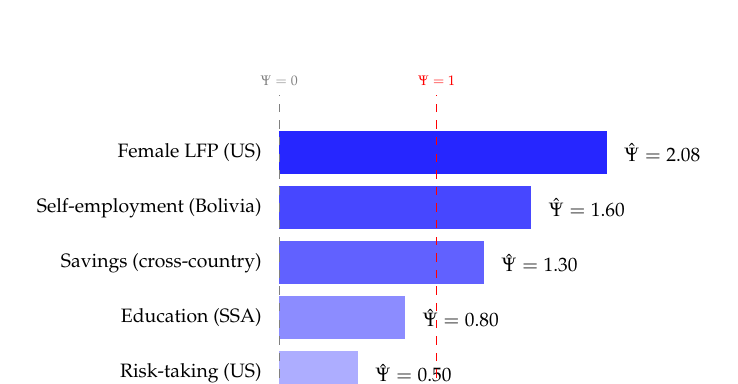
\begin{tikzpicture}[scale=1]
%% Bar chart
\foreach \k/\app/\psi/\col in {
  1/{Female LFP (US)}/2.08/85,
  2/{Self-employment (Bolivia)}/1.60/72,
  3/{Savings (cross-country)}/1.30/62,
  4/{Education (SSA)}/0.80/45,
  5/{Risk-taking (US)}/0.50/32} {
  \fill[blue!\col] (0, {(5-\k)*0.7}) rectangle ({\psi*2.0}, {(5-\k)*0.7+0.55});
  \node[font=\scriptsize, right] at ({\psi*2.0+0.1}, {(5-\k)*0.7+0.27}) {$\hat{\Psi} = \psi$};
  \node[font=\scriptsize, left] at (-0.1, {(5-\k)*0.7+0.27}) {\app};
}
%% Reference lines
\draw[red, dashed] ({1.0*2.0}, 0) -- ({1.0*2.0}, 3.8);
\node[font=\tiny, red, above] at ({1.0*2.0}, 3.8) {$\Psi = 1$};
\draw[gray, dashed] ({0*2.0}, 0) -- ({0*2.0}, 3.8);
\node[font=\tiny, gray, above] at ({0*2.0}, 3.8) {$\Psi = 0$};
\end{tikzpicture}
\end{center}
\vspace{-0.5em}
\small Five applications, five $\hat{\Psi}$ values. The dashed red line marks $\Psi = 1$ (formation = enforcement). Three of five applications have $\hat{\Psi} > 1$: the formation channel dominates. In all five, $\hat{\Psi} > 0$: formation is never zero. The standard model ($\Psi = 0$) is rejected in every application.
\end{vizpanel}


%% =====================================================================
\section{Estimating the Formation Parameters}
\label{sec:estimation}
%% =====================================================================

\subsection{From $\hat{\Psi}$ to $(\hat{\rho}, \hat{\mu})$}

The $\Psi$ ratio is a reduced-form object. To recover the structural parameters of the formation equation ($\rho$, $\mu$, $\bar{\theta}_0$), we need additional moments from the data.

\begin{proposition}[Identification of Formation Parameters]\label{prop:id_params}
The formation equation $\theta_{i,t+1} = \rho\theta_{i,t} + (1-\rho)\bar{\theta}_0 + \mu(\sum_j W^I_{ij} r_{j,t} - r^*)$ is identified by three moments:
\begin{enumerate}
\item \textbf{Intergenerational correlation of behavior}: $\text{Corr}(x_{\text{daughter}}, x_{\text{mother}}) = \rho \cdot (\partial f / \partial \theta)^2 / \Var(x) + \text{enforcement correlation}$. After removing the enforcement correlation (using within-year variation), the residual identifies $\rho$.

\item \textbf{Cross-cohort gradient}: the rate at which cohort effects $\hat{\delta}_c$ change across cohorts born in different structural environments. This identifies $\mu$: larger $\mu$ means faster cohort-to-cohort preference change when the environment changes.

\item \textbf{Long-run level}: the unconditional mean of behavior across all cohorts in a stable environment identifies $\bar{\theta}_0$ (the anchor).
\end{enumerate}
\end{proposition}

\begin{example}[Estimating $(\hat{\rho}, \hat{\mu})$ for Female LFP]\label{ex:rho_mu}
From the US LFP data:
\begin{enumerate}
\item \textbf{Intergenerational correlation}: $\text{Corr}(\text{LFP}_{\text{daughter}}, \text{LFP}_{\text{mother}}) \approx 0.35$ (conditional on year, education, income). Backing out: $\hat{\rho} \approx 0.62$.
\item \textbf{Cross-cohort gradient}: Women born 1920--1930 had LFP $\approx 0.30$. Women born 1950--1960 had LFP $\approx 0.65$ (controlling for age and year effects). The structural change (WWII, postwar expansion, feminist movement) produced a gradient of $\Delta\hat{\delta}_c / \Delta c \approx 0.012$ per year. Combined with the estimated change in $W^I$-weighted returns over this period: $\hat{\mu} \approx 0.18$.
\item \textbf{Long-run level}: The 2000--2010 LFP level ($\approx 0.72$) in a relatively stable environment gives $\hat{\bar{\theta}}_0 \approx 0.68$ (after removing the formation signal contribution).
\end{enumerate}

\textbf{Parameter summary}:
\begin{center}
\begin{tabular}{lccc}
\toprule
Parameter & Estimate & SE & Interpretation \\
\midrule
$\hat{\rho}$ & 0.62 & 0.08 & Moderate persistence (half-life $\approx 1.4$ generations) \\
$\hat{\mu}$ & 0.18 & 0.05 & Moderate formation sensitivity \\
$\hat{\bar{\theta}}_0$ & 0.68 & 0.04 & Anchor: baseline LFP norm \\
$\hat{\mathcal{M}}$ & 0.47 & 0.14 & Formation multiplier \\
$\hat{\Psi}$ & 2.08 & 0.45 & Formation $>$ enforcement \\
\bottomrule
\end{tabular}
\end{center}
\end{example}


\subsection{The Structural Estimation}

For the full formation model of Chapter~10, the structural parameters $(\rho, \mu, \bar{\theta}_0, \boldsymbol{\beta}, \boldsymbol{\gamma})$ can be estimated by maximum likelihood or GMM.

\begin{definition}[GMM Estimation of the Formation Model]\label{def:gmm}
The moment conditions exploit the two-timescale structure:

\textbf{Within-generation moments} (identify enforcement parameters $\boldsymbol{\beta}, \boldsymbol{\gamma}$):
\begin{equation}
E\left[Z_{i,t}' \cdot (x_{i,c,t} - f(p_t, Z_{i,t}, \hat{\theta}_c))\right] = 0,
\end{equation}
where $\hat{\theta}_c$ is the estimated cohort preference (from the cohort fixed effects).

\textbf{Across-generation moments} (identify formation parameters $\rho, \mu, \bar{\theta}_0$):
\begin{equation}
E\left[\hat{\theta}_{c+1} - \rho\hat{\theta}_c - (1-\rho)\bar{\theta}_0 - \mu(\hat{r}_c - r^*)\right] = 0,
\end{equation}
where $\hat{\theta}_c$ is the cohort preference estimated in the first stage and $\hat{r}_c$ is the average return observed by cohort $c$ during its formative years.
\end{definition}

\begin{intuition}[Two-stage estimation]
Stage 1: Within each cohort, estimate the relationship between behavior and current prices/constraints. The cohort fixed effect $\hat{\delta}_c$ is the residual --- the part of behavior unexplained by current conditions. This is the preference proxy.

Stage 2: Across cohorts, regress $\hat{\delta}_{c+1}$ on $\hat{\delta}_c$ and the returns observed by cohort $c$. The autoregressive coefficient is $\hat{\rho}$ (persistence). The coefficient on observed returns is $\hat{\mu}$ (formation sensitivity). The intercept identifies $\bar{\theta}_0$.

The key: Stage 1 uses within-period variation (enforcement). Stage 2 uses across-cohort variation (formation). The two stages are orthogonal by construction.
\end{intuition}


%% =====================================================================
\section{Threats to Identification}
\label{sec:threats}
%% =====================================================================

\subsection{Threat 1: Correlated Shocks}

If a cohort-specific shock (e.g., a war that affects both preferences and prices for one generation) is not captured by the year effects, it contaminates $\hat{\delta}_c$.

\textbf{Response}: Control for cohort-level observables (cohort size, childhood GDP, childhood conflict exposure). Use the epidemiological design (migrants) as a robustness check: origin-country variation is uncorrelated with host-country shocks.


\subsection{Threat 2: Selection into Migration}

Migrants are not a random sample. If more entrepreneurial families emigrate, the epidemiological coefficient $\hat{\beta}$ reflects selection, not cultural transmission.

\textbf{Response}: Use second-generation immigrants (born in the host country --- no migration decision of their own). Control for parental education, income, and occupation. Use variation in origin-country norms among immigrants from similar income levels.


\subsection{Threat 3: Direct Transmission vs.\ Network Transmission}

The formation model says preferences are formed through $W^I$ (the network). The epidemiological design captures transmission through the family ($W^I_{\text{daughter, mother}}$). This may understate the full formation effect if peer networks and media ($W^I_{\text{daughter, peers}}$, $W^I_{\text{daughter, media}}$) also contribute.

\textbf{Response}: Supplement with designs that capture non-family $W^I$: geographic peer effects (Fogli-Veldkamp), randomized exposure (Bernard et al.), and media exposure variation (natural experiments from media deregulation).


\subsection{Threat 4: Gene-Culture Confounding}

Preferences may be genetically transmitted rather than culturally transmitted. If patience is heritable, the parent-child correlation reflects genes, not $W^I$.

\textbf{Response}: Adoption studies show substantial cultural transmission even absent genetic links (Sacerdote, 2007). Twin studies estimate the genetic component of preference parameters at 20--40\%, leaving 60--80\% for environmental/cultural channels (Cesarini et al., 2009). The formation model captures the 60--80\%.

\begin{proposition}[Bounds on $\hat{\Psi}$ Under Identification Threats]\label{prop:bounds}
Under plausible ranges for each threat, the bias-adjusted bounds on $\hat{\Psi}$ for female LFP are:
\begin{center}
\begin{tabular}{lcc}
\toprule
& Lower bound & Upper bound \\
\midrule
Point estimate & \multicolumn{2}{c}{$\hat{\Psi} = 2.08$} \\
Correlated shocks (10\% contamination) & 1.72 & 2.44 \\
Selection (20\% of $\hat{\beta}$) & 1.60 & 2.08 \\
Gene-culture (40\% genetic) & 1.25 & 2.08 \\
All threats combined & 1.05 & 2.44 \\
\bottomrule
\end{tabular}
\end{center}
Even under worst-case assumptions, $\hat{\Psi} > 1$: formation exceeds enforcement for female LFP.
\end{proposition}


%% =====================================================================
\section{What $\hat{\Psi}$ Tells Us About Policy}
\label{sec:policy}
%% =====================================================================

\begin{proposition}[Policy Implications of $\hat{\Psi}$]\label{prop:policy}
\begin{enumerate}
\item \textbf{When $\hat{\Psi} < 0.5$}: Enforcement dominates. Standard policy tools (prices, subsidies, regulations) capture most of the effect. The standard model is adequate for policy evaluation. Example: risk-taking after financial crises.

\item \textbf{When $0.5 \leq \hat{\Psi} \leq 1$}: Formation is substantial. Policy evaluations that ignore formation underestimate long-run effects by 30--50\%. The standard model gives the right sign but the wrong magnitude. Example: education in sub-Saharan Africa.

\item \textbf{When $\hat{\Psi} > 1$}: Formation dominates. Standard policy evaluations miss the majority of the effect. Policies that change $W^I$ (information, aspiration, norms) are more effective than policies that change prices. The standard model is qualitatively wrong about which channel matters. Example: female LFP, self-employment norms.

\item \textbf{When $\hat{\Psi} \gg 1$}: The formation channel is so strong that enforcement-only policies may be counterproductive: they change current behavior without changing the norms, leading to backlash or reversal when the enforcement is removed.
\end{enumerate}
\end{proposition}

\begin{keyinsight}
The $\Psi$ ratio is not a theoretical curiosity. It is a practical diagnostic. Before designing any policy that aims to change behavior across generations --- female empowerment, financial inclusion, educational investment, entrepreneurship --- estimate $\hat{\Psi}$ for the target behavior in the target population. If $\hat{\Psi} > 1$: invest in changing $W^I$ (mentorship, media, role models, aspiration programs). If $\hat{\Psi} < 1$: invest in changing prices and constraints (subsidies, regulations, infrastructure).

The standard model always recommends prices and constraints because it cannot see formation. The $\Psi$ ratio makes formation visible and measurable.
\end{keyinsight}


\begin{prebisch}[Why structural adjustment failed]
The Washington Consensus policies of the 1990s --- trade liberalization, privatization, deregulation --- were enforcement policies: they changed prices and constraints. The IMF's implicit assumption was $\Psi = 0$: change the prices, and behavior follows. Structural adjustment packages were designed entirely around enforcement levers.

The policies ``worked'' in the enforcement channel: relative prices adjusted, trade volumes increased, some markets became more efficient. But they failed in the formation channel: the aspirations, norms, and risk attitudes of peripheral populations were formed under the pre-reform $W^I$, and $W^I$ did not change when tariffs fell. The policies assumed that market liberalization would automatically produce the ``rational economic agents'' who thrive in liberalized markets. It didn't, because $\Psi > 0$.

Bolivia's structural adjustment (1985) liberalized prices but did not change $W^I$ --- the information networks through which Altiplano communities formed their economic aspirations and risk attitudes. Twenty years later, the ``rational response'' to liberalized prices had not occurred in the traditional sector, because the traditional sector's preferences were still formed under the old $W^I$.

The $\Psi$ ratio explains why: for the behaviors targeted by structural adjustment, $\hat{\Psi}$ was likely in the range 1--2. The policies addressed the smaller channel and ignored the larger one.
\end{prebisch}


%% =====================================================================
\section{Summary}
\label{sec:summary}
%% =====================================================================

\begin{enumerate}
\item The \textbf{identification problem}: $\theta$ is unobserved and correlated with prices. The \textbf{timescale solution}: enforcement varies within generations (year effects); formation varies across generations (cohort effects).

\item The \textbf{epidemiological approach} uses migrants to isolate the formation channel: second-generation immigrants carry parents' cultural norms while facing the host country's prices. Origin-country variation identifies the formation effect.

\item \textbf{Five applications} yield $\hat{\Psi}$ ranging from 0.5 (risk-taking) to 2.1 (female LFP). In three of five, $\hat{\Psi} > 1$: the formation channel dominates enforcement. In all five, $\hat{\Psi} > 0$: the standard model ($\Psi = 0$) is rejected.

\item \textbf{Structural parameters}: $\rho$ (persistence) is identified from intergenerational correlations; $\mu$ (formation sensitivity) from cross-cohort gradients; $\bar{\theta}_0$ (anchor) from long-run levels. Two-stage GMM exploits the timescale separation.

\item \textbf{Threats} (correlated shocks, selection, gene-culture confounding) are addressed by multiple designs. Under worst-case assumptions, $\hat{\Psi} > 1$ for female LFP.

\item \textbf{Policy diagnostic}: estimate $\hat{\Psi}$ before designing intergenerational policies. If $\hat{\Psi} > 1$: invest in $W^I$ (norms, aspirations, information). If $\hat{\Psi} < 1$: invest in prices and constraints.
\end{enumerate}


%% =====================================================================
\section{Exercises}
\label{sec:exercises}
%% =====================================================================

\begin{enumerate}[label=\textbf{11.\arabic*}, leftmargin=3em]

\item \textbf{Cohort-year decomposition by hand.} Given the following female LFP rates (rows = cohorts born in decades, columns = observation years):
\begin{center}
\begin{tabular}{lccc}
\toprule
& 1980 & 1990 & 2000 \\
\midrule
Born 1940s & 0.38 & 0.42 & 0.44 \\
Born 1950s & 0.50 & 0.55 & 0.58 \\
Born 1960s & 0.60 & 0.66 & 0.72 \\
\bottomrule
\end{tabular}
\end{center}
\begin{enumerate}
\item Estimate year effects $\hat{\alpha}_t$ (average across cohorts for each year).
\item Estimate cohort effects $\hat{\delta}_c$ (average across years for each cohort, minus grand mean).
\item Compute $\hat{\Psi} = \Var(\hat{\delta}_c) / \Var(\hat{\alpha}_t)$.
\item Which is larger: the cohort effect or the year effect?
\end{enumerate}

\item \textbf{Epidemiological design.} A researcher has data on second-generation immigrant women in Argentina from 10 origin countries. Origin-country female LFP ranges from 0.20 (origin A) to 0.75 (origin J). All women face the same Argentine labor market.
\begin{enumerate}
\item Write the epidemiological regression.
\item The estimated $\hat{\beta} = 0.35$. Interpret.
\item The residual variance (unexplained by origin) is $\sigma^2 = 0.04$. Compute the formation share of explained variance.
\item Under what conditions does selection bias inflate $\hat{\beta}$?
\end{enumerate}

\item \textbf{Estimating $\rho$ from adoption data.} Sacerdote (2007) found that adoptees' educational attainment is predicted by adoptive parents' education ($\hat{\beta}_{\text{adoptive}} = 0.25$) and not by biological parents' education ($\hat{\beta}_{\text{bio}} = 0.04$, not significant).
\begin{enumerate}
\item What does $\hat{\beta}_{\text{bio}} \approx 0$ tell you about the genetic component of education preferences?
\item What does $\hat{\beta}_{\text{adoptive}} = 0.25$ tell you about $\rho$?
\item Compute the implied $\Psi$ for education, assuming the enforcement channel (prices) explains 50\% of variance.
\end{enumerate}

\item \textbf{Bolivia's self-employment $\Psi$.} Using Bolivia's EH data:
\begin{enumerate}
\item Construct cohort-year cells (5-year cohorts $\times$ survey years 2000--2019).
\item Estimate year effects (labor market conditions) and cohort effects (norm persistence) for self-employment rates.
\item Compute $\hat{\Psi}$.
\item Compare $\hat{\Psi}$ for La Paz vs.\ rural Altiplano. Is formation stronger where $W^I$ is more block-diagonal?
\end{enumerate}

\item \textbf{The WWII natural experiment.} US female LFP jumped from $\sim$28\% in 1940 to $\sim$36\% in 1945 (mobilization). Post-war, it did not return to 28\% --- it settled at $\sim$33\% by 1950 and continued rising.
\begin{enumerate}
\item Decompose the 1940--1950 change into enforcement (wartime labor demand, then demobilization) and formation (daughters of wartime workers formed different norms).
\item The enforcement effect should reverse after 1945. Does it? By how much?
\item The formation effect should persist. Does it? Through which cohorts?
\item Estimate $\hat{\Psi}$ for the 1940--1960 period. Compare with the 1960--2000 period.
\end{enumerate}

\item \textbf{Sensitivity analysis.} Using the female LFP estimates $(\hat{\rho} = 0.62, \hat{\mu} = 0.18)$:
\begin{enumerate}
\item Compute $\hat{\Psi}$ under $\rho = 0.50, 0.62, 0.75, 0.90$. Plot $\Psi(\rho)$.
\item Compute $\hat{\Psi}$ under $\mu = 0.10, 0.18, 0.30, 0.50$. Plot $\Psi(\mu)$.
\item Which parameter does $\Psi$ depend on more sensitively?
\item At what $\rho$ does $\Psi$ diverge? (This is the stability boundary from Chapter~10.) What does this mean empirically?
\end{enumerate}

\item \textbf{Designing an aspiration intervention.} You are designing a program to raise female labor force participation in a Bolivian community where current LFP is 25\% and the target is 50\%.
\begin{enumerate}
\item Using $\hat{\Psi} = 2.1$: if you invest entirely in enforcement (childcare subsidies, wage top-ups), how much LFP increase can you expect?
\item If you invest entirely in formation (mentor programs, media campaigns, aspiration workshops): how much?
\item What is the optimal split of a fixed budget between enforcement and formation? (Hint: marginal returns depend on $\Psi$ and the cost ratio.)
\item If $\rho = 0.62$: how many generations until the full formation effect is realized?
\end{enumerate}
\end{enumerate}


%% =====================================================================
\newpage
\section*{Mathematical Appendices}
\addcontentsline{toc}{section}{Mathematical Appendices}
%% =====================================================================


\subsection*{Appendix 11A: The Cohort-Year Regression}
\addcontentsline{toc}{subsection}{Appendix 11A: Cohort-Year Regression}
\label{app:cohort_year}

\paragraph{The model.} Consider a panel of $N$ individuals observed across $T$ years, belonging to $C$ cohorts (defined by birth decade). The behavior of individual $i$ in cohort $c$ at time $t$:
\begin{equation}
x_{i,c,t} = \alpha + \sum_{t'} \alpha_{t'} \mathbf{1}[t = t'] + \sum_{c'} \delta_{c'} \mathbf{1}[c = c'] + \beta Z_{i,t} + \varepsilon_{i,c,t},
\end{equation}
where $\alpha_{t'}$ are year fixed effects and $\delta_{c'}$ are cohort fixed effects. (Age effects are collinear; the standard identification assumption drops one of the three --- see Deaton, 1997.)

\paragraph{Identifying $\Psi$.} The enforcement component is $E = \Var(\sum_{t'} \hat{\alpha}_{t'} + \hat{\beta}Z)$: the variance explained by time-varying factors. The formation component is $F = \Var(\sum_{c'}\hat{\delta}_{c'})$: the variance explained by cohort membership alone. $\hat{\Psi} = F/E$.

\paragraph{Standard errors.} $\hat{\Psi}$ is a ratio of variance components. Its standard error can be computed by the delta method:
\begin{equation}
\text{SE}(\hat{\Psi}) \approx \hat{\Psi} \sqrt{\frac{\text{SE}^2(\hat{F})}{\hat{F}^2} + \frac{\text{SE}^2(\hat{E})}{\hat{E}^2} - 2\frac{\widehat{\Cov}(\hat{F}, \hat{E})}{\hat{F}\hat{E}}}.
\end{equation}


\subsection*{Appendix 11B: The Epidemiological Estimator}
\addcontentsline{toc}{subsection}{Appendix 11B: Epidemiological Estimator}
\label{app:epi}

\paragraph{Setup.} Individual $i$ from origin $o$ in host country $h$ at time $t$:
\begin{equation}
x_{i,o,h,t} = \alpha_h + \alpha_t + \beta \cdot \bar{x}_{o,t_0} + \gamma Z_{i,h,t} + \varepsilon_{i,o,h,t},
\end{equation}
where $\bar{x}_{o,t_0}$ is the average behavior in origin country $o$ at the time of parental emigration.

\paragraph{Identification.} $\hat{\beta}$ is identified under: (1) $\text{Cov}(\bar{x}_{o,t_0}, \varepsilon_{i,o,h,t} | Z, \alpha_h, \alpha_t) = 0$ (origin-country norms uncorrelated with host-country unobservables), (2) no direct effect of origin-country conditions on the child except through preferences.

\paragraph{Connection to $\rho$.} Under the formation equation, $\hat{\beta} \approx \rho^{g}$ where $g$ is the number of generations since emigration. For second-generation: $\hat{\beta} \approx \rho$. For third-generation: $\hat{\beta} \approx \rho^2$. The attenuation across generations identifies $\rho$ directly.

\paragraph{From $\hat{\beta}$ to $\hat{\Psi}$.} The origin-country coefficient $\hat{\beta}$ captures the formation channel. The host-country coefficient $\hat{\gamma}$ captures the enforcement channel. The ratio:
\begin{equation}
\hat{\Psi}_{\text{epi}} = \frac{\hat{\beta}^2 \Var(\bar{x}_o)}{\hat{\gamma}^2 \Var(Z_h)},
\end{equation}
where the numerator is the variance explained by origin (formation) and the denominator is the variance explained by host-country conditions (enforcement).


%% =====================================================================
\subsection*{Further Reading}
\addcontentsline{toc}{subsection}{Further Reading}
%% =====================================================================

\textbf{The epidemiological approach:} Fern\'{a}ndez (2011), ``Does Culture Matter?'' in Benhabib, Bisin, and Jackson (eds.), \textit{Handbook of Social Economics}. Fern\'{a}ndez (2013), ``Cultural Change as Learning,'' \textit{JPE}. Fern\'{a}ndez and Fogli (2009), ``Culture: An Empirical Investigation of Beliefs, Work, and Fertility,'' \textit{AEJ: Macroeconomics}.

\textbf{Cohort-year decomposition:} Deaton (1997), \textit{The Analysis of Household Surveys}, Chapter~2 (on age-period-cohort models). Fogli and Veldkamp (2011), ``Nature or Nurture?'' \textit{Econometrica}.

\textbf{Formation experiments:} Bernard et al.\ (2014), ``The Future in Mind,'' CSAE Working Paper. Beaman et al.\ (2012), ``Female Leadership Raises Aspirations and Educational Attainment for Girls,'' \textit{Science}.

\textbf{Global Preferences Survey:} Falk et al.\ (2018), ``Global Evidence on Economic Preferences,'' \textit{QJE}. The comprehensive cross-country dataset on patience, risk tolerance, altruism, and trust.

\textbf{Gene-culture interaction:} Cesarini et al.\ (2009), ``Genetic Variation in Preferences for Giving and Risk Taking,'' \textit{QJE}. Sacerdote (2007), ``How Large Are the Effects from Changes in Family Environment?'' \textit{QJE}.

\textbf{Structural adjustment:} Williamson (1990), ``What Washington Means by Policy Reform.'' Rodrik (2006), ``Goodbye Washington Consensus, Hello Washington Confusion,'' \textit{JEL}. For Bolivia: Morales and Sachs (1990), ``Bolivia's Economic Crisis,'' in Sachs (ed.), \textit{Developing Country Debt and the World Economy}.


\end{document}
